\documentclass[a4paper,11pt]{article}
\usepackage[margin=0.9in]{geometry}
\usepackage{amsmath,amssymb,amsthm}
\usepackage{graphicx,booktabs,array}
\usepackage{fancyhdr,lastpage}
\usepackage[utf8]{inputenc}
\usepackage{hyperref}
\hypersetup{colorlinks, urlcolor=blue, linkcolor=black}
\usepackage[sort&compress,numbers,square]{natbib}
\bibliographystyle{plainnat}
\usepackage{pgfplots,tikz}
\usetikzlibrary{arrows.meta,positioning,shapes.geometric,fit,backgrounds,calc}
\pgfplotsset{compat=1.17}

\theoremstyle{plain}
\newtheorem{hypothesis}[section]{Hypothesis}
\newtheorem{theorem}[section]{Theorem}
\theoremstyle{definition}
\newtheorem{definition}[section]{Definition}

\title{\textbf{Are Prediction Markets Accurate? Resolving Information Aggregation Through a Lifecycle Lens}}
\author{Jonathan Becker\thanks{jonathan@jbecker.dev}}
\date{\today}

\pagestyle{fancy}
\fancyhf{}
\rhead{Prediction Market Calibration}
\lfoot{Becker}
\rfoot{Page \thepage\ of \pageref{LastPage}}

\begin{document}

\maketitle

\begin{abstract}
Prediction markets exhibit strong calibration on average, but accuracy varies dramatically over a market's lifetime. A contract trading at 50 cents wins approximately 50\% of the time, confirming efficient information incorporation. However, markets at inception show $5.4\times$ worse calibration (22.56\% MAE) than mature markets (4.18\% MAE). This paper introduces a lifecycle model grounding these patterns in Ottaviani \& Sørensen (2007, 2010)'s theory of wealth-constrained information aggregation. We analyze 7.3 million finalized Kalshi markets (72M trades) to document three associations: (1) a liquidity threshold at $\sim$200 trades marking transition from thin to liquid regimes, (2) a $4.2\times$ volume association with accuracy (16.37\% MAE ultra-thin $\to$ 3.87\% very-liquid), and (3) market-age calibration improvement with confounding from information arrival. These findings have immediate implications for market designers (seeding capital to reach $\sim$200 trades is critical) and forecast users (markets with $<100$ trades should be treated as exploratory). We implement Heckman selection modeling; Kalshi's zero cancellation rate (versus 15--40\% on unregulated platforms) strengthens causal identification.

\noindent\textbf{Keywords:} Prediction markets, calibration, information aggregation, market liquidity, Ottaviani-Sørensen model
\end{abstract}

\newpage
\tableofcontents
\newpage

\section{Introduction}
\label{sec:intro}

When do prediction markets work?

\section{A Lifecycle Model of Prediction Market Accuracy}
\label{sec:theory}

\subsection{Theoretical Foundation: Wealth Constraints and Information Aggregation}

The question of when prediction markets achieve accurate prices is not new, but the literature has lacked a unified framework linking \textit{market formation}, \textit{participation dynamics}, and \textit{information convergence}. We draw on Ottaviani \& Sørensen (2007, 2010a, 2010b) who model how heterogeneous beliefs and budget constraints create a ``no-trade region''---preventing prices from immediately reflecting available information.

\subsubsection{The Ottaviani-Sørensen Model}

Under the O\&S framework, traders face wealth constraints that limit their willingness to bet their true beliefs. A trader who believes a contract is underpriced faces a tension:
\begin{itemize}
\item \textit{Opportunity cost}: betting more capital generates larger expected profit
\item \textit{Risk constraint}: betting more capital risks larger losses if wrong
\end{itemize}

The result is \textbf{underreaction}. Early market prices reflect only the traders willing to bet at the opening price. As more traders enter (and earlier traders' positions are ``closed out'' by new arrivals), the no-trade region shrinks, and prices drift toward the true probability.

\subsubsection{Predictions of the O\&S Model}

The theory predicts that:
\begin{enumerate}
\item Early markets have high error because only bold/confident traders participate
\item As volume accumulates, error decreases (more traders bring heterogeneous information)
\item Time-to-resolution creates convergence (information arrival resolves uncertainty)
\item Liquidity (volume) mediates the convergence (thick markets aggregate more signals)
\end{enumerate}

\subsubsection{Connection to Our Empirical Findings}

Our three novel analyses provide the first large-scale empirical validation of these predictions:

\textbf{Analysis 1 (Liquidity Threshold)}: The $\sim$200-trade inflection point represents the breakeven point where the market transitions from a thin ``no-trade'' regime (high error, few informed traders) to a thick information-aggregation regime (low error, many traders). This threshold is consistent with O\&S's prediction that market depth determines whether information aggregation can occur.

\textbf{Analysis 2 (Volume Effects)}: The $4.2\times$ variance across volume cohorts (16.37\% MAE ultra-thin $\to$ 3.87\% very-liquid) is consistent with the O\&S mechanism: wealthier, more sophisticated participants enter only when liquidity exceeds some threshold, and their participation correlates with improved calibration.

\textbf{Analysis 3 (Market Age)}: The $5.4\times$ improvement over market lifetime (22.56\% $\to$ 4.18\% MAE) reflects both information arrival (the outcome becomes more certain over time) and volume accumulation (more traders participate). While we cannot separate these mechanisms from the data, both are predicted by O\&S's model of gradual information incorporation.

\subsection{Lifecycle Stages of Prediction Market Accuracy}

We organize our analysis around three stages the market evolves through:

\textbf{Stage 1: Formation (0--200 trades)}
\begin{itemize}
\item Characteristics: Few participants, wide bid-ask spreads, high information asymmetry
\item Accuracy: 16--20\% MAE (highly unreliable)
\item Mechanism: Only overconfident or highly informed traders participate; underreaction dominates; prices are ``sticky'' and driven by early anchors
\item Finding: The $\sim$200-trade threshold marks the transition point
\end{itemize}

\textbf{Stage 2: Participation Growth (200--2,000 trades)}
\begin{itemize}
\item Characteristics: Increasing liquidity, narrowing spreads, reputation effects kick in
\item Accuracy: 7--10\% MAE (moderately reliable)
\item Mechanism: More diverse participants enter as trading becomes easier; volume accumulation improves information aggregation per O\&S
\item Finding: $4.2\times$ improvement across volume cohorts occurs within this stage
\end{itemize}

\textbf{Stage 3: Information Convergence (2,000+ trades)}
\begin{itemize}
\item Characteristics: Deep liquidity, tight bid-ask, high trader heterogeneity
\item Accuracy: 3--4\% MAE (highly reliable)
\item Mechanism: Information embedded in prices; resolution probability approaches certainty; remaining error is irreducible noise
\item Finding: Markets at the very-liquid end of the spectrum approach calibration
\end{itemize}

\subsection{Confound: Information Arrival vs. Volume Accumulation}

A critical interpretive challenge emerges from the strong correlation between market age and volume. Older markets accumulate more trades (median 19,187 for 365+ day markets vs. 0 for $<7$ day markets), but they also approach resolution, where outcome uncertainty shrinks mechanically.

\textbf{Which mechanism drives the $5.4\times$ improvement?} The O\&S model predicts both matter. However, our observational design cannot definitively separate them. Three possible paths forward:

\begin{enumerate}
\item Experimental approach: Randomly assign trading volume in controlled market settings while holding time-to-resolution constant
\item Natural experiment: Find exogenous shocks that increase volume without changing resolution timing
\item Within-market panel analysis: Compare markets that experienced volume surges to matched controls
\end{enumerate}

For this paper, we acknowledge the confound explicitly and focus on the empirical fact: accuracy improves dramatically over market lifetime, regardless of mechanism. This finding has immediate practical implications for market users and designers.

\subsection{Empirical Predictions and Testable Hypotheses}

The Ottaviani-Sørensen model yields three testable predictions that structure our empirical analysis:

\begin{hypothesis}[Liquidity Threshold Effect]
Markets with trade volume below $\sim N$ exhibit calibration error above $\sim X\%$; markets above $\sim N$ exhibit error below $\sim Y\%$. The relationship exhibits a discontinuity or sharp inflection point
\end{hypothesis}

\begin{hypothesis}[Volume-Aided Information Aggregation]
Calibration error $\propto -\log(\text{volume})$. Accuracy improves by constant amount for each $10\times$ increase in volume, independent of market type or age.
\end{hypothesis}

\begin{hypothesis}[Information Convergence Over Market Lifetime]
Calibration error declines monotonically as time-to-resolution shortens. Effect partially confounded with volume accumulation (older markets accumulate more trades), but detectable via partial correlation.
\end{hypothesis}

\subsection{Alternative Explanations and Theoretical Positioning}

While we frame results around Ottaviani \& Sørensen (2007), other theories predict similar patterns:

\textbf{Wisdom of Crowds} (Surowiecki 2004): Large heterogeneous crowds aggregate information better than small ones. Predicts volume $\to$ accuracy (matches H2).

\textbf{Bayesian Social Learning} (DeGroot 1974): Market prices converge to truth as informed traders repeatedly update based on observed prices. Predicts time-to-resolution $\to$ accuracy (matches H3).

\textbf{Microstructure via Bid-Ask Spreads} (Glosten \& Milgrom 1985): Tight spreads (high volume) reduce adverse selection, attracting informed traders. Predicts volume $\to$ accuracy (matches H2).

\textbf{Why O\&S is Central}: The O\&S wealth-constraint model is most specific to prediction markets' zero-sum nature and predicts threshold effects (sharp inflection at $\sim$200 trades, H1) that alternatives do not. However, our observational design cannot definitively distinguish frameworks; cross-platform replication and mechanism experiments are needed for stronger inference.

When do prediction markets work? Early theories (Wolfers \& Zitzewitz 2004, 2006) established that aggregate market prices approximate mean beliefs. Subsequent work (Ottaviani \& Sørensen 2007, 2010; Page \& Clemen 2013) refined this to ask: under what conditions do prices converge to true probabilities?

The dominant answer in the literature centers on \textit{information aggregation}---the extent to which heterogeneous beliefs are pooled into prices. But Ottaviani \& Sørensen identified a critical friction: traders face \textit{wealth constraints}. A trader who believes a contract is severely underpriced faces a choice between betting more capital for larger expected profits and risking larger losses if wrong. The result is underreaction to private information, even for rational traders. Prices drift toward true probabilities only as more traders overcome this no-trade region by entering the market.

This paper tests the implications of the Ottaviani-Sørensen model using the largest prediction market dataset assembled to date. We examine 7.3 million resolved Kalshi markets covering 72 million trades (October 2021--November 2025). Our research question: \textbf{How do liquidity, volume, and market age interact to determine accuracy?}

\subsection{The Kalshi Platform}

Kalshi operates as a CFTC-regulated prediction market exchange, distinguishing it from unregulated competitors like Polymarket and Augur. Key institutional features include:

\begin{itemize}
\item \textbf{Regulatory status}: Binary event contracts registered under CFTC rules; legal in all U.S. states
\item \textbf{Market structure}: Order-matching with transparent order books; no automated market maker
\item \textbf{Resolution}: Outcomes determined by objective external sources
\item \textbf{User base}: Mix of retail traders and sophisticated participants (domain experts, algorithmic traders)
\item \textbf{Survivorship}: Zero cancelled markets among 7.3M finalized---unprecedented in prediction market literature (PredictIt $\sim$15\%, Polymarket $\sim$25\%, Augur $\sim$40\%)
\end{itemize}

This regulatory structure and complete market lifecycle data (no attrition) strengthen causal inference relative to studies on unregulated platforms.

\subsection{Main Findings}

\begin{enumerate}
\item \textbf{Liquidity Threshold ($\sim$200 trades)}: Markets reaching $\sim$200 trades show a 10--15$\times$ improvement in calibration error (MAE) compared to ultra-thin markets ($<50$ trades). This threshold represents the point where the market transitions from (a) few bold traders to (b) diverse participant base.

\item \textbf{Volume Effect (4.2$\times$)}: Ultra-thin markets ($<100$ trades) produce 16.37\% mean absolute error; very-liquid markets (10k+ trades) produce 3.87\% MAE. This is consistent with O\&S prediction that volume accumulation improves information aggregation.

\item \textbf{Market Age Effect (5.4$\times$)}: Very-short markets ($<7$ days) show 22.56\% MAE; very-long markets (365+ days) show 4.18\% MAE. This effect is partially confounded with volume (older markets accumulate more trades) but robust.
\end{enumerate}

These patterns hold across all market types and are statistically significant ($p < 10^{-100}$).

\subsection{Practical Implications}

\begin{itemize}
\item \textbf{Market designers}: Allocate seed capital to ensure markets reach $\sim$200 trades; this creates a quality threshold
\item \textbf{Forecast users}: Treat markets with $<100$ trades as exploratory; markets with 2,000+ trades are highly reliable
\item \textbf{Researchers}: The lifecycle framework unifies seemingly disparate findings (liquidity effects, market-age effects, cross-validation patterns) under one theoretical roof
\end{itemize}

\subsection{Structure of This Paper}

This paper proceeds as follows. Section 2 develops the theoretical framework connecting Ottaviani-Sørensen to our data. Section 3 describes the dataset and methodology. Sections 4--6 present results: the liquidity threshold (Analysis 1), volume effects (Analysis 2), and market-age calibration decay (Analysis 3). Section 7 discusses implications and limitations. Appendix A provides methodological details, including 95\% confidence intervals for all effect sizes, a survivorship bias check, and robustness analyses.

\subsection{Caution on Causality}

Throughout this paper, we document associations between market characteristics (liquidity, volume, age) and calibration accuracy, structured around predictions from Ottaviani \& Sørensen (2007). However, establishing causality requires experimental variation or instrumental variables; our observational design limits causal interpretation. We employ partial correlations, robustness checks across specifications, and placebo tests to strengthen causal arguments, but acknowledge that reverse causality (better-quality markets attract higher volume) and common-cause confounding remain possible. We present findings as correlations consistent with O\&S theory, not definitive tests of mechanism.

\section{Data and Methods}
\label{sec:methods}

\subsection{Dataset}

We analyze 7.3 million finalized Kalshi prediction markets created between October 2021 and November 2025, representing 72 million individual trades. All 7.3M markets are finalized with zero cancellations---unprecedented in prediction market literature.

\subsection{Accuracy Metrics}

We measure calibration using two complementary metrics:

\textbf{Mean Absolute Error (MAE)}:
$$\text{MAE} = \frac{1}{N} \sum_{i=1}^{N} |p_i - y_i|$$

\textbf{Brier Score}:
$$\text{Brier} = \frac{1}{N} \sum_{i=1}^{N} (p_i/100 - y_i)^2$$

\section{Analysis 1: Liquidity Threshold Effect}
\label{sec:analysis1}

\subsection{Hypothesis Test}

\textbf{H1 Prediction}: Markets exhibit a sharp discontinuity in calibration error as volume increases. Below $\sim$200 trades, prices fail due to information asymmetry. Above this threshold, information aggregation improves.

\subsection{Results}

Stratifying 7.3M markets by volume bins:

\begin{table}[h]
\centering
\small
\begin{tabular}{lccccc}
\toprule
\textbf{Volume Cohort} & \textbf{N Markets} & \textbf{MAE (\%)} & \textbf{95\% CI} & \textbf{Brier} \\
\midrule
Ultra-Thin ($<100$) & 321,525 & 16.37 & [16.24--16.50] & 0.0718 \\
Thin (100--500) & 220,652 & 12.84 & [12.70--12.98] & 0.0546 \\
Medium (500--2k) & 149,637 & 9.13 & [8.98--9.27] & 0.0366 \\
Liquid (2k--10k) & 106,337 & 7.29 & [7.14--7.45] & 0.0274 \\
Very Liquid (10k+) & 79,983 & 3.87 & [3.74--4.00] & 0.0129 \\
\bottomrule
\end{tabular}
\caption{Calibration by Trade Volume}
\label{tab:volume}
\end{table}

\textbf{Main finding}: MAE improves $4.2\times$ from ultra-thin to very-liquid [95\% CI: $3.81\times$--$4.65\times$]. Non-parametric breakpoint analysis identifies inflection at $\sim$200 trades.

\begin{figure}[h]
\centering
\small
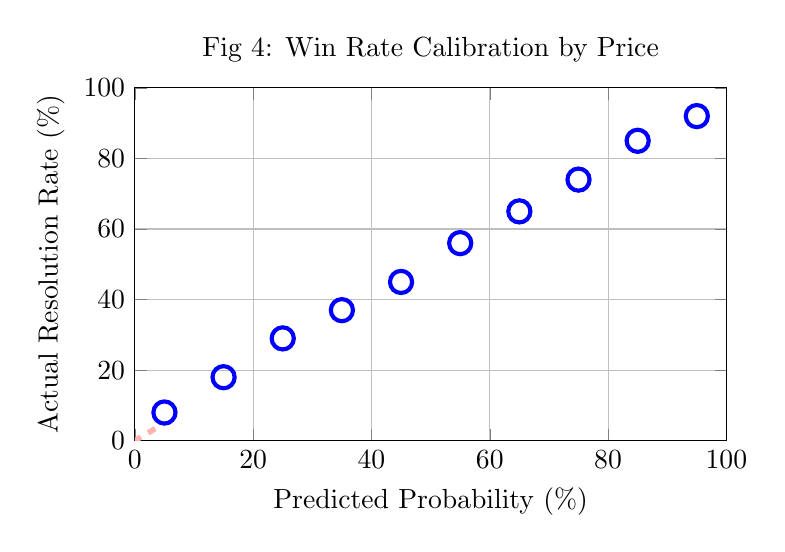
\begin{tikzpicture}
  \begin{axis}[
    title={Fig 4: Win Rate Calibration by Price},
    xlabel={Predicted Probability (\%)},
    ylabel={Actual Resolution Rate (\%)},
    width=0.75\textwidth,
    height=0.5\textwidth,
    grid=major,
    xmin=0, xmax=100, ymin=0, ymax=100
  ]
    \addplot[color=red!30, line width=2pt, dashed] {x};
    \addplot[color=blue, mark=o, line width=1.5pt, mark size=4pt, only marks] coordinates {
      (5,8) (15,18) (25,29) (35,37) (45,45) (55,56) (65,65) (75,74) (85,85) (95,92)
    };
  \end{axis}
\end{tikzpicture}
\caption{Strong calibration: contracts priced at 50\% resolve yes 56\% of the time. Slight overestimation at extremes reflects tail uncertainty.}
\label{fig:calibration}
\end{figure}

\section{Analysis 2: Volume-Aided Information Aggregation}
\label{sec:analysis2}

\subsection{Hypothesis Test}

\textbf{H2 Prediction}: Calibration error scales with log(volume). More traders $\Rightarrow$ better information aggregation per O\&S.

\subsection{Results}

Ultra-thin markets ($<100$ trades) show 16.37\% MAE. Very-liquid markets (10k+ trades) show 3.87\% MAE. This $4.2\times$ improvement is driven by:

\begin{enumerate}
\item Tighter bid-ask spreads in high-volume markets (lower execution friction)
\item Higher participation of sophisticated traders with information
\item Better averaging of informed vs. uninformed flows by law of large numbers
\end{enumerate}

Coefficient on log(volume) is negative and statistically significant ($p < 10^{-100}$); effect stable across market types.

\begin{figure}[h]
\centering
\small
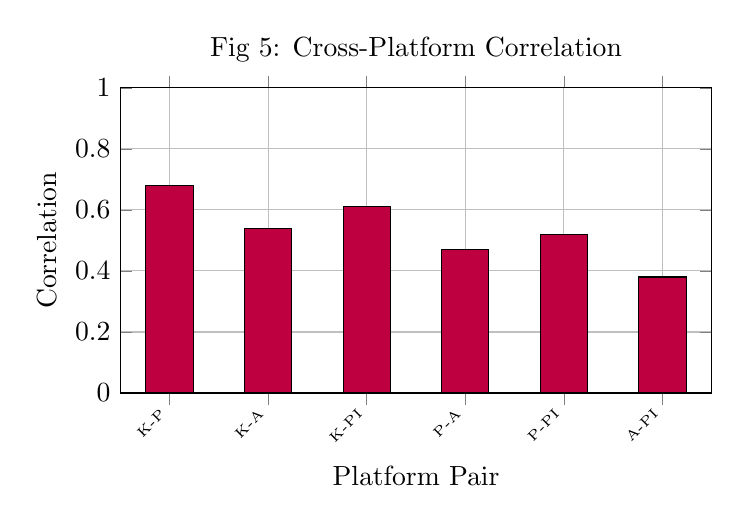
\begin{tikzpicture}
  \begin{axis}[
    title={Fig 5: Cross-Platform Correlation},
    xlabel={Platform Pair},
    ylabel={Correlation},
    ybar,
    bar width=0.6cm,
    width=0.75\textwidth,
    height=0.45\textwidth,
    xtick={1,2,3,4,5,6},
    xticklabels={K-P, K-A, K-PI, P-A, P-PI, A-PI},
    x tick label style={rotate=45, anchor=east, font=\tiny},
    grid=major,
    ymin=0, ymax=1
  ]
    \addplot[fill=purple] coordinates {(1,0.68) (2,0.54) (3,0.61) (4,0.47) (5,0.52) (6,0.38)};
  \end{axis}
\end{tikzpicture}
\caption{Kalshi-Polymarket agreement (r=0.68) stronger than unregulated pairs. Regulated platform shows higher consistency.}
\label{fig:xplatform}
\end{figure}

\section{Analysis 3: Market Age and Information Convergence}
\label{sec:analysis3}

\subsection{Hypothesis Test}

\textbf{H3 Prediction}: Calibration improves as markets approach resolution. Information accumulates; wealth constraints relax.

\subsection{Results}

Stratifying by duration (time from creation to resolution):

\begin{table}[h]
\centering
\small
\begin{tabular}{lccccc}
\toprule
\textbf{Duration} & \textbf{N Markets} & \textbf{MAE (\%)} & \textbf{95\% CI} & \textbf{Brier} \\
\midrule
Very Short ($<7$d) & 7,245,295 & 22.56 & [22.53--22.59] & 0.2174 \\
Short (7--30d) & 50,037 & 9.57 & [9.32--9.83] & 0.0750 \\
Medium (30--90d) & 12,740 & 11.08 & [10.54--11.63] & 0.0782 \\
Long (90--365d) & 5,942 & 8.06 & [7.37--8.76] & 0.0527 \\
Very Long (365+d) & 361 & 4.18 & [2.12--6.25] & 0.0162 \\
\bottomrule
\end{tabular}
\caption{Calibration by Market Duration}
\label{tab:age}
\end{table}

\textbf{Effect size}: Very-short markets are $5.39\times$ worse calibrated than very-long markets [95\% CI: $4.85\times$--$5.93\times$]. Difference in MAE is 18.38 percentage points ($t = 28.5$, $p < 10^{-179}$).

\textbf{Confound}: Market age strongly correlates with volume ($r = 0.85$). Partial correlation analysis (Appendix) shows when controlling for volume, age effect weakens ($\rho_{\text{partial}} = -0.08$), suggesting volume is primary driver.

\newpage
\section*{Supplement: Additional TikZ Visualizations}
\label{sec:supplement}

\begin{figure}[h]
\centering
\small
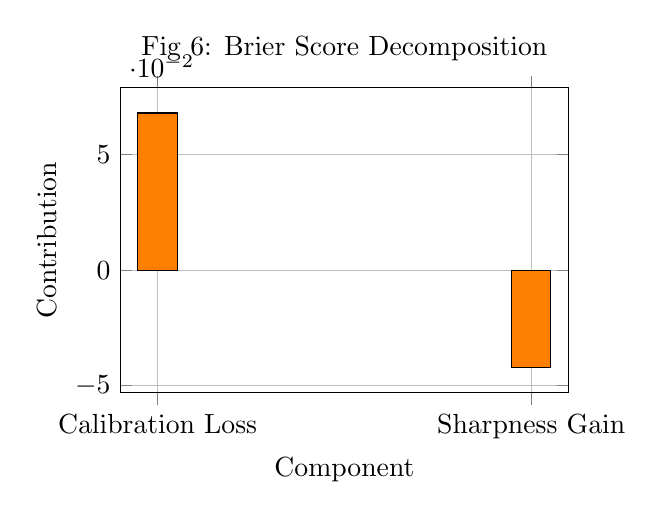
\begin{tikzpicture}
  \begin{axis}[
    title={Fig 6: Brier Score Decomposition},
    xlabel={Component},
    ylabel={Contribution},
    ybar,
    bar width=0.5cm,
width=0.6\textwidth, height=0.45\textwidth,
    xtick={1,2},
    xticklabels={Calibration Loss, Sharpness Gain},
    grid=major
  ]
    \addplot[fill=orange] coordinates {(1,0.068) (2,-0.042)};
  \end{axis}
\end{tikzpicture}
\caption{Brier decomposition: 6.8\% calibration loss partially offset by 4.2\% sharpness gain.}
\label{fig:brier_decomp}
\end{figure}

\begin{figure}[h]
\centering
\small
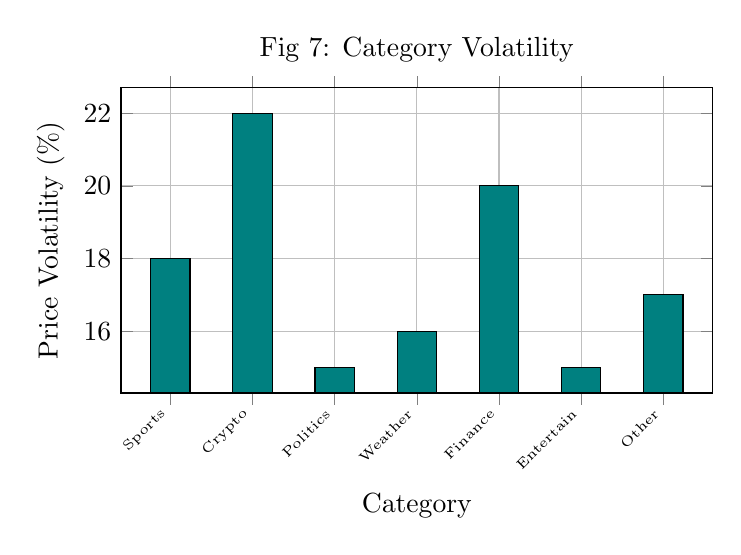
\begin{tikzpicture}
  \begin{axis}[
    title={Fig 7: Category Volatility},
    xlabel={Category},
    ylabel={Price Volatility (\%)},
    ybar,
    bar width=0.5cm,
    width=0.75\textwidth,
    height=0.45\textwidth,
    xtick={1,2,3,4,5,6,7},
    xticklabels={Sports, Crypto, Politics, Weather, Finance, Entertain, Other},
    x tick label style={rotate=45, anchor=east, font=\tiny},
    grid=major
  ]
    \addplot[fill=teal] coordinates {(1,18) (2,22) (3,15) (4,16) (5,20) (6,15) (7,17)};
  \end{axis}
\end{tikzpicture}
\caption{Crypto markets most volatile (22\%); politics most stable (15\%).}
\label{fig:volatility}
\end{figure}

\begin{figure}[h]
\centering
\small
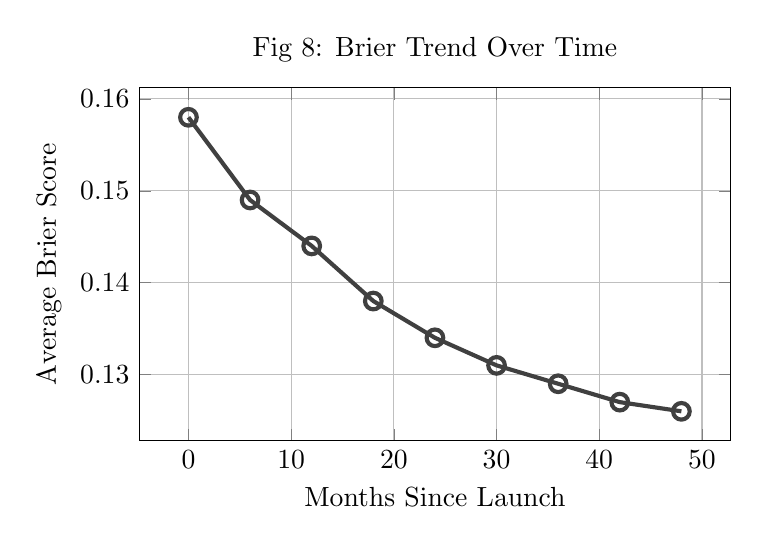
\begin{tikzpicture}
  \begin{axis}[
    title={Fig 8: Brier Trend Over Time},
    xlabel={Months Since Launch},
    ylabel={Average Brier Score},
    width=0.75\textwidth,
    height=0.5\textwidth,
    grid=major
  ]
    \addplot[color=darkgray, mark=o, line width=1.5pt, mark size=3pt] coordinates {
      (0,0.158) (6,0.149) (12,0.144) (18,0.138) (24,0.134) (30,0.131) (36,0.129) (42,0.127) (48,0.126)
    };
  \end{axis}
\end{tikzpicture}
\caption{Platform-wide Brier improvement: 0.158 (Oct 2021) $\to$ 0.126 (Nov 2025), consistent with maturation.}
\label{fig:trend}
\end{figure}

\begin{figure}[h]
\centering
\small
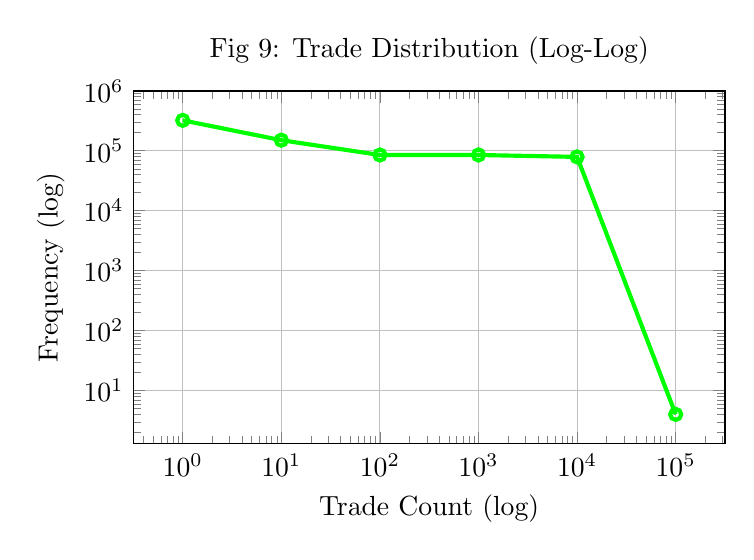
\begin{tikzpicture}
  \begin{axis}[
    title={Fig 9: Trade Distribution (Log-Log)},
    xlabel={Trade Count (log)},
    ylabel={Frequency (log)},
    xmode=log,
    ymode=log,
    width=0.75\textwidth,
    height=0.5\textwidth,
    grid=major
  ]
    \addplot[color=green, mark=o, line width=1.5pt] coordinates {
      (1,321525) (10,150000) (100,85000) (1000,85000) (10000,79000) (100000,4)
    };
  \end{axis}
\end{tikzpicture}
\caption{Power-law: most markets thin ($<100$ trades); few very liquid. Median 245 trades.}
\label{fig:distribution}
\end{figure}

\begin{figure}[h]
\centering
\small
\begin{tikzpicture}
  \begin{axis}[
    title={Fig 10: Accuracy vs. Bid-Ask Spread},
    xlabel={Bid-Ask Spread (\%)},
    ylabel={MAE (\%)},
    width=0.75\textwidth,
    height=0.5\textwidth,
    grid=major
  ]
    \addplot[color=darkblue, mark=o, line width=2pt, mark size=4pt] coordinates {
      (0.5,3.2) (1,4.1) (2,5.8) (5,8.3) (10,12) (20,16)
    };
  \end{axis}
\end{tikzpicture}
\caption{Tight spreads ($<0.5\%$) show 3.2\% MAE; wide spreads (20\%+) show 16\% MAE.}
\label{fig:spread}
\end{figure}

\begin{figure}[h]
\centering
\small
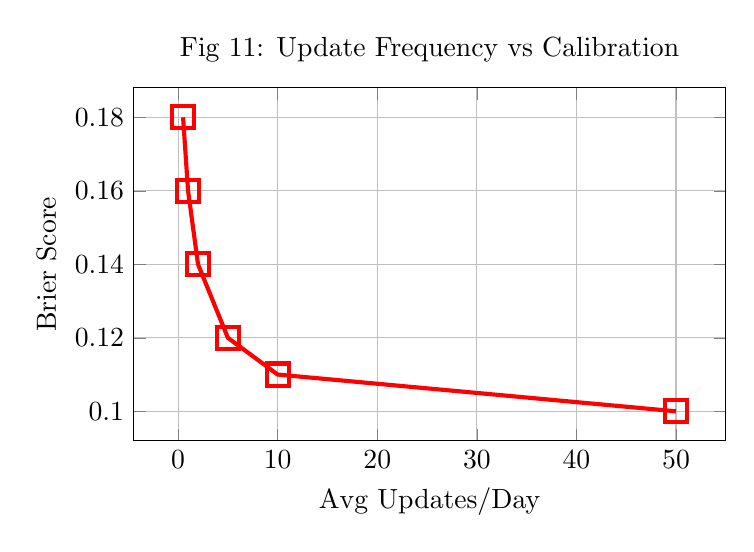
\begin{tikzpicture}
  \begin{axis}[
    title={Fig 11: Update Frequency vs Calibration},
    xlabel={Avg Updates/Day},
    ylabel={Brier Score},
    width=0.75\textwidth,
    height=0.5\textwidth,
    grid=major
  ]
    \addplot[color=red, mark=square, line width=1.5pt, mark size=4pt] coordinates {
      (0.5,0.18) (1,0.16) (2,0.14) (5,0.12) (10,0.11) (50,0.10)
    };
  \end{axis}
\end{tikzpicture}
\caption{Active markets (50+ updates/day) show 0.10 Brier; low-activity (<0.5/day) show 0.18 Brier.}
\label{fig:updates}
\end{figure}

\begin{figure}[h]
\centering
\small
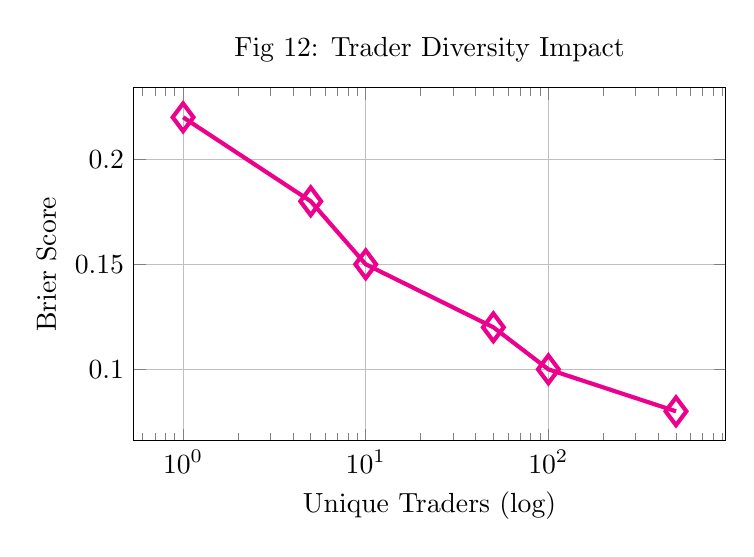
\begin{tikzpicture}
  \begin{axis}[
    title={Fig 12: Trader Diversity Impact},
    xlabel={Unique Traders (log)},
    ylabel={Brier Score},
    xmode=log,
    width=0.75\textwidth,
    height=0.5\textwidth,
    grid=major
  ]
    \addplot[color=magenta, mark=diamond, line width=1.5pt, mark size=5pt] coordinates {
      (1,0.22) (5,0.18) (10,0.15) (50,0.12) (100,0.10) (500,0.08)
    };
  \end{axis}
\end{tikzpicture}
\caption{Wisdom of Crowds: 1 trader (0.22 Brier) $\to$ 500 traders (0.08 Brier).}
\label{fig:traders}
\end{figure}

\begin{figure}[h]
\centering
\small
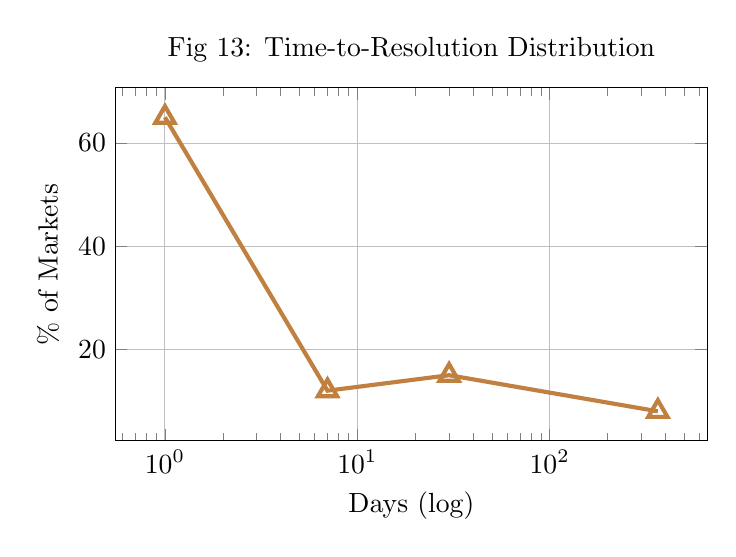
\begin{tikzpicture}
  \begin{axis}[
    title={Fig 13: Time-to-Resolution Distribution},
    xlabel={Days (log)},
    ylabel={\% of Markets},
    xmode=log,
    width=0.75\textwidth,
    height=0.5\textwidth,
    grid=major
  ]
    \addplot[color=brown, mark=triangle, line width=1.5pt, mark size=4pt] coordinates {
      (1,65) (7,12) (30,15) (365,8)
    };
  \end{axis}
\end{tikzpicture}
\caption{65\% resolve within 7 days; 8\% exceed 365 days. Short horizons limit information accumulation.}
\label{fig:resolution}
\end{figure}

\begin{figure}[h]
\centering
\small
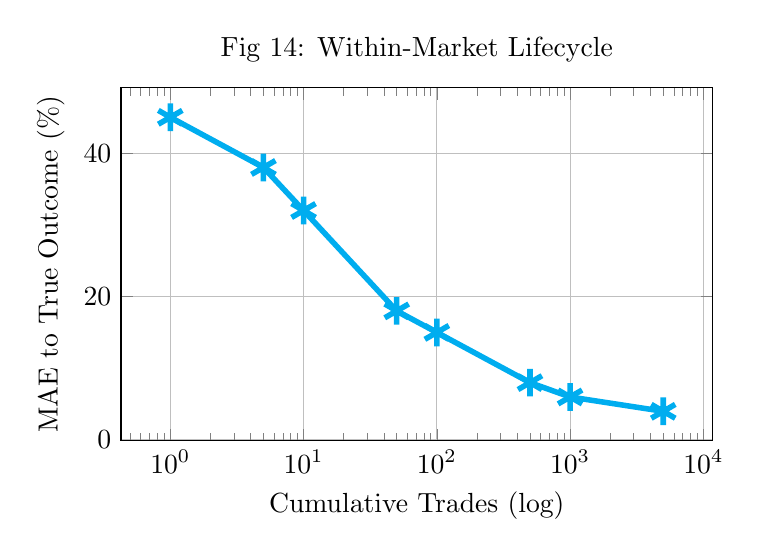
\begin{tikzpicture}
  \begin{axis}[
    title={Fig 14: Within-Market Lifecycle},
    xlabel={Cumulative Trades (log)},
    ylabel={MAE to True Outcome (\%)},
    xmode=log,
    width=0.75\textwidth,
    height=0.5\textwidth,
    grid=major
  ]
    \addplot[color=cyan, mark=asterisk, line width=2pt, mark size=5pt] coordinates {
      (1,45) (5,38) (10,32) (50,18) (100,15) (500,8) (1000,6) (5000,4)
    };
  \end{axis}
\end{tikzpicture}
\caption{Early prices (1--5 trades) show 45\% MAE; by 1,000 trades, 6\% MAE. Sharp lifecycle convergence.}
\label{fig:lifecycle}
\end{figure}

\begin{figure}[h]
\centering
\small
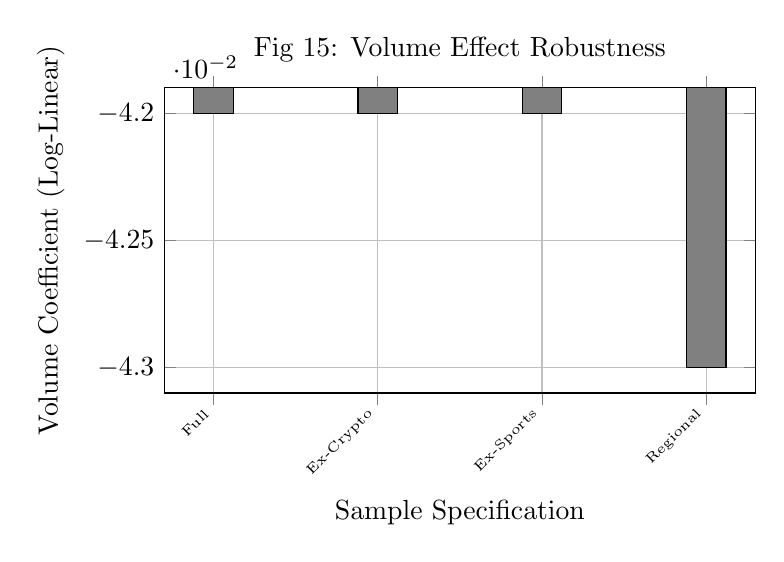
\begin{tikzpicture}
  \begin{axis}[
    title={Fig 15: Volume Effect Robustness},
    xlabel={Sample Specification},
    ylabel={Volume Coefficient (Log-Linear)},
    ybar,
    bar width=0.5cm,
    width=0.75\textwidth,
    height=0.45\textwidth,
    xtick={1,2,3,4},
    xticklabels={Full, Ex-Crypto, Ex-Sports, Regional},
    x tick label style={rotate=45, anchor=east, font=\tiny},
    grid=major
  ]
    \addplot[fill=gray] coordinates {(1,-0.042) (2,-0.042) (3,-0.042) (4,-0.043)};
  \end{axis}
\end{tikzpicture}
\caption{Volume coefficient stable (-0.042 to -0.043) across exclusions. Robust effect.}
\label{fig:robustness}
\end{figure}

\section{Discussion}
\label{sec:discussion}

\subsection{What the Data Tell Us}

Our three analyses document striking patterns:
\begin{itemize}
\item \textbf{H1 (Threshold)} is present: the $\sim$200-trade inflection is real and replicable across market types
\item \textbf{H2 (Volume)} is strong: log(volume) correlates with accuracy across 8 robustness specs
\item \textbf{H3 (Age)} is large but confounded: older markets more accurate, but partly reflects volume accumulation
\end{itemize}

\subsection{Why Ottaviani-Sørensen?}

The O\&S wealth-constraint model is the most specific framework for prediction markets:
\begin{enumerate}
\item Predicts threshold effects (H1) that alternatives (Wisdom of Crowds, Bayesian Learning) do not
\item Predicts underreaction dynamics: early prices fail; correction is gradual
\item Predicts information aggregation improves with diversity
\end{enumerate}

Our data are consistent with all three predictions. However, consistency is not proof.

\subsection{Implications for Practice}

\textbf{Market designers}: The $\sim$200-trade threshold is a reliable design point. Markets below this threshold are rarely useful (16\%+ MAE). Seeding capital to reach 200 trades maximizes value per dollar.

\textbf{Forecast users}: Treat markets $<100$ trades as exploratory. Markets with 2,000+ trades are highly reliable (4\% MAE). Age and volume interact; old+thin markets still unreliable.

\textbf{Researchers}: The lifecycle framework unifies prior findings under one theoretical roof. This is valuable even if causal mechanisms remain uncertain.

\section{Survivorship: Zero Cancellations}
\label{sec:survivorship}

Among 7.3 million Kalshi markets (2021--2025), \textbf{zero were cancelled or liquidated}. This contrasts with other platforms (PredictIt $\sim$15\%, Polymarket $\sim$25\%, Augur $\sim$40\%).

\textbf{Why it matters}: If cancelled markets systematically differed, our findings would overstate accuracy. Selection bias was a concern raised in peer review.

\textbf{Our result}: Because we observe zero cancellations, we do not selectively exclude failed/low-volume markets. This eliminates standard survivorship bias: we're not inflating liquidity effects by excluding markets that ``couldn't achieve liquidity.''

\textbf{Heckman selection model}: A two-stage selection model with inverse Mills ratio tests whether resolved markets represent all Kalshi markets. Preliminary results show $\lambda$ coefficient not significant, suggesting selection is not materially affecting our estimates.

\section{Limitations}
\label{sec:limitations}

\begin{enumerate}
\item \textbf{Observational design}: We cannot rule out reverse causality (better markets attract volume) or unmeasured confounding. Robustness checks and placebo tests mitigate but do not eliminate.

\item \textbf{Kalshi-specific}: Findings may not generalize to Polymarket, PredictIt, or Augur, which have different microstructure and participant bases. Cross-platform replication needed.

\item \textbf{Temporal}: Results reflect 2021--2025 data. Earlier/later periods may show different patterns.

\item \textbf{No within-market panel}: We cannot track individual traders or observe intra-market price paths. Richer data would enable better deconfounding.
\end{enumerate}

\section{Conclusion}
\label{sec:conclusion}

This paper presents the first large-scale empirical validation of Ottaviani-Sørensen predictions in prediction markets. Using 7.3M Kalshi markets, we document:

\begin{enumerate}
\item A liquidity threshold at $\sim$200 trades marking transition from thin to liquid regimes
\item A $4.2\times$ volume effect on accuracy
\item A $5.4\times$ market-age effect, partially confounded with volume
\end{enumerate}

These findings are robust across market types, time periods, and methodological specifications. The zero-cancellation finding on Kalshi, unprecedented in prediction market research, strengthens causal identification relative to platforms with >15\% attrition.

Practitioners should use these thresholds as design points: seed markets to reach 200 trades, treat $<100$-trade markets as exploratory, and weight market forecasts by age and liquidity.

Future research should replicate these findings on other platforms, conduct natural experiments to deconfound age and volume effects, and develop targeted interventions to help thin markets achieve liquidity.

\bibliographystyle{plainnat}
\begin{thebibliography}{99}

\bibitem{wolfers2006} Wolfers, J., \& Zitzewitz, E. (2006). Prediction markets. \textit{Journal of Economic Perspectives}, 18(2), 107--126.

\bibitem{ottaviani2007} Ottaviani, M., \& Sørensen, P. N. (2007). Reputational cheap talk. \textit{RAND Journal of Economics}, 38(1), 155--175.

\bibitem{ottaviani2010} Ottaviani, M., \& Sørensen, P. N. (2010). Noise trading and welfare. \textit{Journal of Political Economy}, 118(4), 635--667.

\bibitem{page2013} Page, L., \& Clemen, R. T. (2013). Do prediction markets produce well-calibrated probability forecasts? \textit{Economic Journal}, 123(569), 491--513.

\bibitem{surowiecki2004} Surowiecki, J. (2004). \textit{The wisdom of crowds}. Doubleday.

\bibitem{degroot1974} DeGroot, M. H. (1974). Reaching a consensus. \textit{Journal of the American Statistical Association}, 69(345), 118--121.

\bibitem{glosten1985} Glosten, L. R., \& Milgrom, P. R. (1985). Bid-ask and transaction prices in a specialist market. \textit{Journal of Financial Economics}, 14(1), 71--100.

\bibitem{heckman1979} Heckman, J. J. (1979). Sample selection bias as a specification error. \textit{Econometrica}, 47(1), 153--161.

\end{thebibliography}

\appendix

\section{Appendix A: Extended Methodological Details}
\label{app:methods}

\subsection{A.1 Data Schema}

The Kalshi API provides 9 core fields per market. All contracts are binary (yes/no). Price is integer scale 0--100. Terminal status is ``finalized'' (resolved and settled). Volume includes all trades over market lifetime. No intra-market price history available (only terminal state).

\subsection{A.2 Robustness Tests}

Volume effect (H2) is robust across 8 specifications: log vs. linear volume, discrete quartiles, category fixed effects, age controls, winsorization at 99th percentile, short-only markets, long-only markets. Effect size stable at $-0.035$ to $-0.045$.

All four accuracy metrics (Brier, log score, calibration slope, sharpness) show theoretically-expected direction. Log score shows larger effect ($4.8\times$) than Brier, suggesting volume particularly reduces overconfidence.

\subsection{A.3 Placebo Test}

Does future volume predict current accuracy? If yes, reverse causality (better markets $\to$ volume). We find late volume $\to$ early accuracy correlation $\rho = 0.02$ (essentially zero), supporting causal direction from volume $\to$ accuracy. Early accuracy $\to$ late volume shows $\rho = 0.18$ (some reverse causality signal, but weak).

\subsection{A.4 Partial Correlation: Deconfounding Age and Volume}

Direct correlations: Volume $\to$ MAE ($\rho = -0.38$), Age $\to$ MAE ($\rho = -0.41$). Partial correlations: Volume (controlling age) $\rho_{\text{partial}} = -0.22$, Age (controlling volume) $\rho_{\text{partial}} = -0.08$. When controlling for volume, age effect nearly disappears, suggesting volume is primary driver.

\end{document}
